\documentclass{article}

\usepackage[%
    left=0.5in,%
    right=0.5in,%
    top=0.5in,%
    bottom=0.5in,%
]{geometry}%
\usepackage{minitoc}
\usepackage{multicol}
\usepackage{graphicx}
\usepackage{fixltx2e}
\usepackage{listings}
\usepackage{amsmath}
\usepackage{color}
\usepackage{hyperref}
    \hypersetup{ colorlinks = true, linkcolor = blue }
\usepackage{blindtext}
\definecolor{lightgray}{gray}{0.9}
\graphicspath{ {./} }

\newcommand{\inlinecode}[2]{\colorbox{lightgray}{\lstinline
[language=#1]$#2$}}
\newcommand{\worddef}[1]{\hyperref[sec:reference]{\textit{#1}}}

\begin{document}

\tableofcontents

\newpage

\section{Why Measure Software?}

\begin{itemize}
  \item To determine the quality of the current product or process and to make informed comparisons
  \item To predict qualities of a product/process
  \item To improve quality of a product/process (often continuously – \worddef{kaizen})
\end{itemize}

\section{Metrics}

\subsection{Example metrics}
\begin{itemize}
  \item Error rates / Defect rates 
  \item A defect is a failure to do something 
  \item An error is a wrong result or illegal action 
  \item Code generation rates. Measured by: per \textbf{person}, per \textbf{team}, per \textbf{project}. Will involve \textbf{aggregation} – see later
  \item Errors should be categorized by origin, type etc.
\end{itemize}

\subsection{Main objectives of software quality metrics}

\begin{itemize}
  \item Facilitate management control, planning and managerial intervention. Based on deviations of actual 
  \begin{itemize}
    \item performance from planned.
    \item timetable and budget performance from planned. 
  \end{itemize}
  \item 2. Identify situations for development or maintenance process improvement (preventive or corrective actions). Based on:
  \begin{itemize}
    \item Accumulation of metrics information regarding the performance of teams, units, etc.
  \end{itemize}
\end{itemize}

\subsection{Software quality metrics — Requirements}

\begin{flushleft}
General	requirements:
\begin{itemize}
  \item Relevant
  \item Valid
  \item Reliable
  \item Comprehensive 
  \item Mutually exclusive
\end{itemize}
Operative requirements:
\begin{itemize}
  \item Easy and simple 
  \item Does not require independent data collection 
  \item Immune to biased interventions by interested parties
\end{itemize}
\end{flushleft}

\subsection{Metrics evaluations}

\begin{flushleft}
Metrics can be evaluated on:
\begin{itemize}
  \item \textbf{Products}: Explicit results of software development activities. Deliverables, documentation, other artifacts produced
  \item \textbf{Process}: Activities	related	to	production	of	software
  \item \textbf{Resource}: Inputs into the software development activities, such as hardware, knowledge, people.
\end{itemize}
\end{flushleft}

\subsection{Process metrics}

\begin{flushleft}
Rates of production / productivity, quality of estimates, burn down rate (project velocity), refactoring rate. These can lead to \textbf{long term process improvement} by driving reflection on the process and suggestions for improvement
\end{flushleft}

\subsection{Product metrics}

\begin{flushleft}
Error densities, complexity measures, code quality measures, speed and memory measures, code profiles etc, track potential risks, uncover problem areas, Adjust workflow or tasks. They \textbf{evaluate teams ability to control quality}
\end{flushleft}

\subsection{Types of measures}
\begin{itemize}
  \item Direct: Cost, effort, LOC, speed, memory
  \item Indirect: functionality, quality, efficiency, reliablity, maintainability 
\end{itemize}


\subsection{Size oriented metrics}
\begin{itemize}
  \item Size of software produced
  \item LOC - Lines of Code or KLOC - 1000 Lines of code
  \item SLOC statement lines of code (no whitespace)
  \item Number of function points (NFP)
  \item Open used as part of density CONT
\end{itemize}

\subsection{Process metrics categories}
\begin{itemize}
  \item Software oricess quality metrics: Error density, severity metrics
  \item Software process timetable, error removal effectiveness and productivity metrics.
\end{itemize}

\section{Process metrics}


\subsection{Definitions}

\begin{flushleft}
  \item NCE = total detected by code inspections and testing.
  \item NDE = total errors detected in the development process.
  \item WCE = weighted NCE
  \item WDE = weighted NDE
  \item MSOT = Milestones completed on time.
  \item MS = Total number of milestones.
  \item TCDAM = Total Completion Delays (days, weeks, etc.) for all milestones
  \item NYF = number software failures detected during a year of maintenance service.
  \item WYF = weighted number of software failures detected during a year of maintenance service.
  \item DevH = Total working hours invested in the development of the software system.
  \item ReKLOC = Number of thousands of reused lines of code.
  \item ReDoc = Number of reused pages of documentation.
  \item NDoc = Number of pages of documentation
\end{flushleft}

\subsection{Error density metrics}

\begin{itemize}  
  \item CED (Code error density) $CED = NCE / KLOC$
  \item DED (Development error density) $DED = NDE /KLOC $
  \item WCED (Weighted code error density) $WCDE = WCE / KLOC$
  \item WDED (Weighted development error density) $WDED = WDE / KLOC$
  \item WCEF (Weighted code errors per function point) $WCEF = WCE / NFP $
  \item WDEF (Weighted development errors per function point) $WDEF = WDE / NFP$
\end{itemize}

\subsection{Error severity metrics}

\begin{itemize}
  \item ASCE (Average severity of code errors) $ ASCE = WCE / NCE$
  \item ASDE (Average severity of developmment errors) $ASDE = WDE / NDE$
\end{itemize}

\subsection{Software process timetable metrics}

\begin{itemize}
  \item TTO (Time table observance) $ TTO = MSOT / MS $
  \item ADMC (Average delay of milestone completion) $ADMC = TCDAM / MC$
\end{itemize}

\subsection{Error removal effectiveness metric}

\begin{itemize}
  \item DERE (Development errors removal effectiveness) $ DERE = NDE / (NDE + NFY)$
  \item DWERE (Development weighted erros removal effectiveness) $ DWERE = WDE / (WDE + WYF)$ 
\end{itemize}

\subsection{Software process productivity metrics}

\begin{itemize}
  \item DevP (Development productivity) $DevP = DevH / KLOC$
  \item FDevP (Function point development productivity) $ FDevP = DevH / NFP$
  \item CRe (Code reuse) $Cre = ReKLOCK / KLOCK$
  \item DocRe (Documentation reuse) $DocRe = ReDoc / NDoc$
\end{itemize}

\section{LOC based metrics}

\begin{itemize}
  \item Easy	to	use	and compute	
  \item Language \&	programmer	dependent	
  \item Can	be	counter-productive	if	used	as	a	basis	for	reward! (Program can be written in more lines of code and made overly complex)
\end{itemize}

\subsection{Complexity Metrics}

\begin{itemize}
  \item  LOC	-	a	function	of	complexity
  \item  Language	and	programmer	dependent
  \item Halstead’s	Software	Science	(entropy	measures)
  \begin{itemize}
    \item $n_{1}$	-	number	of	distinct	operators
    \item  $n_{2}$	-	number	of	distinct	operands	
    \item  $N_{1}$	-	total	number	of	operators
    \item  $N_{2}$	-	total	number	of	operands
  \end{itemize}
\end{itemize}

\subsection{Halstead’s Metrics}

\begin{itemize}
  \item Program length: $N = N_{1} + N_{2}$
  \item Program vacabulary: $n = n_{1} + n_{2}$
  \item Estimated	length: $N \text{\^{}} \: = \: n_{1} * log_{2}n_{1} + n_{2} * log_{2}n_{2} $ (Close	estimate	of	length	for	well	structured	programs	)
  \item Purity ratio $PR \: = N \text{\^{}} / N$
\end{itemize}

\section{Program complexity}

\begin{itemize}
  \item Volume: $V = N \log_2 n$ (Number	of	bits	to	provide	a	unique	designator	for	each	of	the	n	items	in	the	program	vocabulary
)
  \item Difficulty: $D = (n_{1} / 2) * (N_{2} / n_{2})$
  \item Program effort = $E = D * V$ (good	measure	of	program	understandability)
\end{itemize}

\section{McCabe’s Complexity Measures}

\begin{itemize}
  \item McCabe’s	metrics	are	based	on	a	control	flow	representation	of	the	program.	
  \item  A	program	graph	is	used	to	depict	control	flow.	
  \item  Nodes	represent	\textbf{processing	tasks}	(one	or	more	code	statements)	
  \item  Edges	represent	\textbf{control	flow	between	nodes}
\end{itemize}

\subsection{Flow Graph Notation}

\begin{center}
  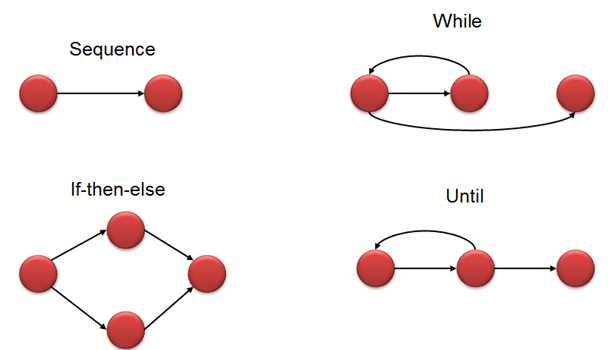
\includegraphics[scale=0.5]{mccabe_flow.png}
\end{center}

\subsection{Cyclomatic Complexity}

\begin{itemize}
  \item Set	of	independent	paths	through	the	graph	(basis	set)	
  \item $V(G) = E - N + 2$
  \begin{itemize}
    \item E	is	the	number	of	flow	graph	edges
    \item N is the number of edges
  \end{itemize}
  \item $V(G)	=	P	+	1$
  \begin{itemize}
    \item  P	is	the	number	of	predicate	nodes	(branching)	
  \end{itemize}
\end{itemize}

\subsection{Meaning}

\begin{itemize}
  \item V(G)	is	the	number	of	(enclosed)	regions/areas	of	the	planar	graph	
  \item  Number	of	regions	increases	with	the	number	of	decision	paths	and	loops	
  \item  This	is	a	quantitative	measure	of	the	number	of	tests	needed		
  \item  It	correlates	very	well	with	the	rate	of	errors	
  \item  Experimental	data	shows	value	of	V(G)	should	be	no	more	then	10	-	testing	is	very	difficult	above	this	value
\end{itemize}

\section{McClure’s Complexity Metric}

\begin{flushleft}
Complexity =	$C	+	V$
\begin{itemize}
  \item  C	is	the	number	of	comparisons	in	a	module
  \item  V	is	the	number	of	control	variables	referenced	in	the	module
\end{itemize}
decisional complexity. Similar to McCabe's but with regard to control variables
\end{flushleft}

\section{Metrics and Software Quality (FURPS)}
\begin{itemize}
  \item Functionality		-	features	of	system	
  \item  Usability	–	aesthesis,	documentation	
  \item  Reliability	–	frequency	of	failure,	security	
  \item  Performance	–	speed,	throughput	
  \item  Supportability	–	maintainability
\end{itemize}

\section{Measures of Software Quality}

\begin{itemize}
  \item Measures of Software QualityCorrectness	–	degree	to	which	a	program	operates	according	to	specification
  \item Mintainability	–	degree	to	which	a	program	is	open	to	change
  \item Integrity	-	degree	to	which	a	program	is	resistant	to	outside	attack	
  \item Usability	–	easiness	to	use
\end{itemize}

\pagebreak

\section*{Reference section} \label{sec:reference}
\begin{description}
	\item[measure] \hfill \\ A quantitative indication of extent, amount, dimension, capacity, or size of some attribute of a product or process. for example: Lines of code (LOC), Number of errors
	\item[metric] \hfill \\ quantitative measure of degree to which a system, component or process possesses a given attribute. That is to say a “derived measure.” May involve “guesstimates” where human processes are concerned. for example: Error density.
	\item[kaizen] \hfill \\ An approach to \textbf{continuous} organization improvement with emphasis on continuous measure and understanding of process.
\end{description}
\end{document}
